\documentclass{article}
\usepackage[utf8]{inputenc}
\usepackage{amssymb,amsmath,amsthm}
\usepackage{enumerate}
\usepackage[left=.75 in, right=.75 in,top=.75 in, bottom=.75 in]{geometry}
\usepackage{fancyhdr}
\usepackage{bm}
\usepackage{graphicx}
\usepackage{subfigure}
\usepackage{parskip}

\graphicspath{ {img/} }

\pagestyle{fancy}
\fancyhf{}
\fancyhead[L]{Statistical Modeling and Analysis of SST-Pyr Synapses}
\fancyhead[R]{Page \thepage}
\renewcommand{\headrulewidth}{0.4pt}

\setlength{\parskip}{2mm}

\def\Pr{\textbf{Pr }}
\def\Var{\textbf{Var}}
\def\E{\textbf{E}}

\newcommand{\rv}[1] {
\text{$\bm{#1}$}
}

\DeclareMathOperator{\bern}{Bern}

\providecommand{\norm}[1]{\left\Vert#1\right\Vert}

\author{Taisuke Yasuda}

\begin{document}

\begin{center}
  {\LARGE Statistical Modeling and Analysis of SST-Pyr Synapses} \\
  \vspace{10pt}
  {Taisuke Yasuda \qquad 11/28/2016}
\end{center}

\section{Research Goal}
When we sampled postsynaptic responses from SST-Pyr synapses, the resulting distribution had an oddly long tail relative to the expectation of the distribution. That is, these cells have a very high failure rate, yet exhibit responses of very high amplitude. The research problem of this paper is to explain how postsynaptic response amplitudes that are much higher than the average amplitude are achieved.

\begin{figure}[h]
  \caption{A typical distribution with high failure rate and high maximum amplitude}
  \centering
  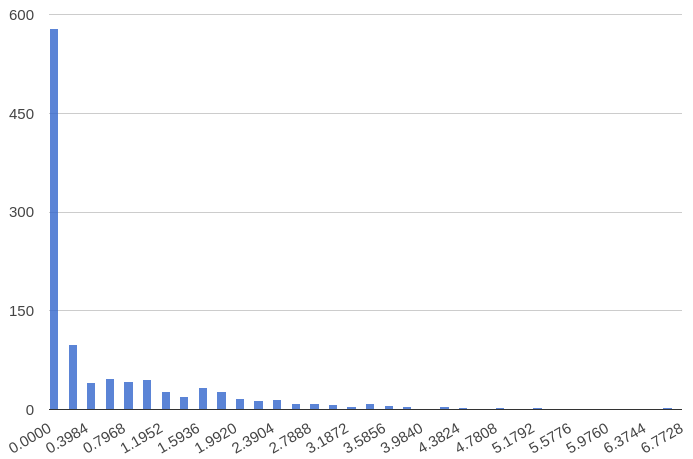
\includegraphics[width=0.5\textwidth]{typical-hist}
\end{figure}

\section{Results}
\subsection{Summary}
Our studies show that the observed data is best explained by a distribution of postsynaptic amplitudes over contacts with a high variance. We first find that the simple model obtained by assuming that the release probabilities, which we refer to as $p$, and response amplitudes, which we refer to as $q$, of each contact are the same does not sufficiently explain the data obtained from the experiment. We then find that when we take the response amplitudes across contacts to have a uniform distribution with large width parameter, we recover a model that explains the data well, as measured by QQ plots.

\subsection{The statistical model}
We seek to explain the underlying mechanics of the observed distribution by constructing a statistical model that sufficiently matches the observed distribution. The model we build is the following:
\[
  \rv{A} = \sum_{j=1}^N \rv{A}_j, \rv{A}_j = \begin{cases}
    N(q_j,\sigma_j^2) & \text{if $\rv{S}_j = 1$} \\
    0 & \text{if $\rv{S}_j = 0$}
  \end{cases}, \rv{S}_j = \bern(p_j)
\]
In this model, $\rv{A}$ is the random variable we observe, $\rv{A}_j$ are the latent random variables that represent the release amplitudes of each contact, and $\rv{S}_j$ are the latent random variables that represent the release success of each contact. We assume that the $\rv{A}_j$ are independent. If the contact $\rv{A}_j$ releases, which it does with probability $p_j$, then we observe a response assumed to be normally distributed with mean $q_j$ and variance $\sigma_j^2$. Otherwise, we observe a response of $0$ from $\rv{A}_j$. Finally, we observe the sum of the $\rv{A}_j$, which gives $\rv{A}$.

\subsection{Analysis of the constant parameter model}
Note that in the above model, we have reduced the distribution to a choice of four parameters, $N$, the number of contacts, $q$, the vector of the average response at each contact, $p$, the vector of the release probability at each contact, and $\sigma^2$, the vector of the variance of response at each contact. As an initial analysis of the model, we assume that all the release probabilities, response amplitudes, and variances at each contact are the same. Although we do not expect a model assuming this to sufficiently explain the observed data, we use this analysis to gain a feel for the data.

Given this assumption, we can estimate the parameters $p$, $q$, and $\sigma$ from the statistics of the data to be
\[
  p = 1 - \sqrt[N]{p_f},\ q = \frac{\overline{\mu}}{Np},\ \sigma^2 = \frac{s^2}{Np} - q^2 + q^2p,
\]
where $p_f$ is the failure rate, $\overline{\mu}$ is the sample mean, and $s^2$ is the sample variance (details in the technical appendix). We do not attempt to estimate $N$ and instead we simulate the model over a range of reasonable values of $N$, as suggested by data from reconstructions of SST-Pyr synapses.

\begin{figure}
  \subfigure[A good fit]{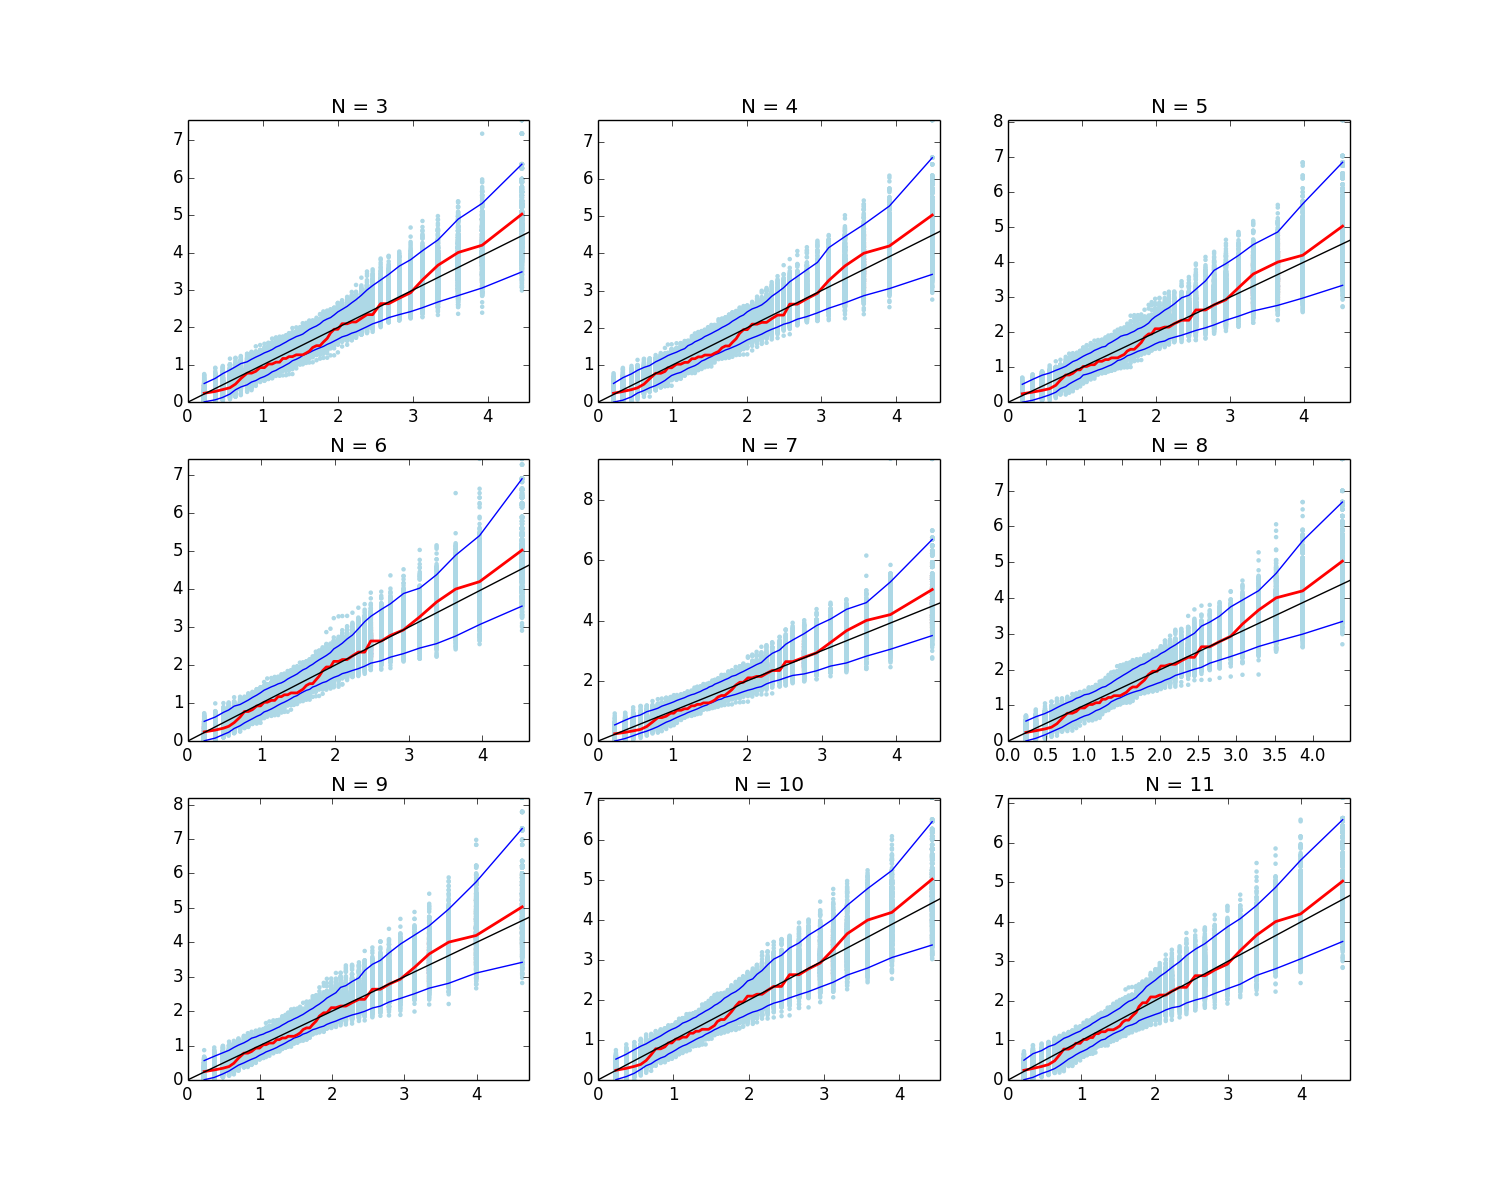
\includegraphics[width=0.5\textwidth]{11sept2015e-9-qq}}
  \hfill
  \subfigure[A bad fit]{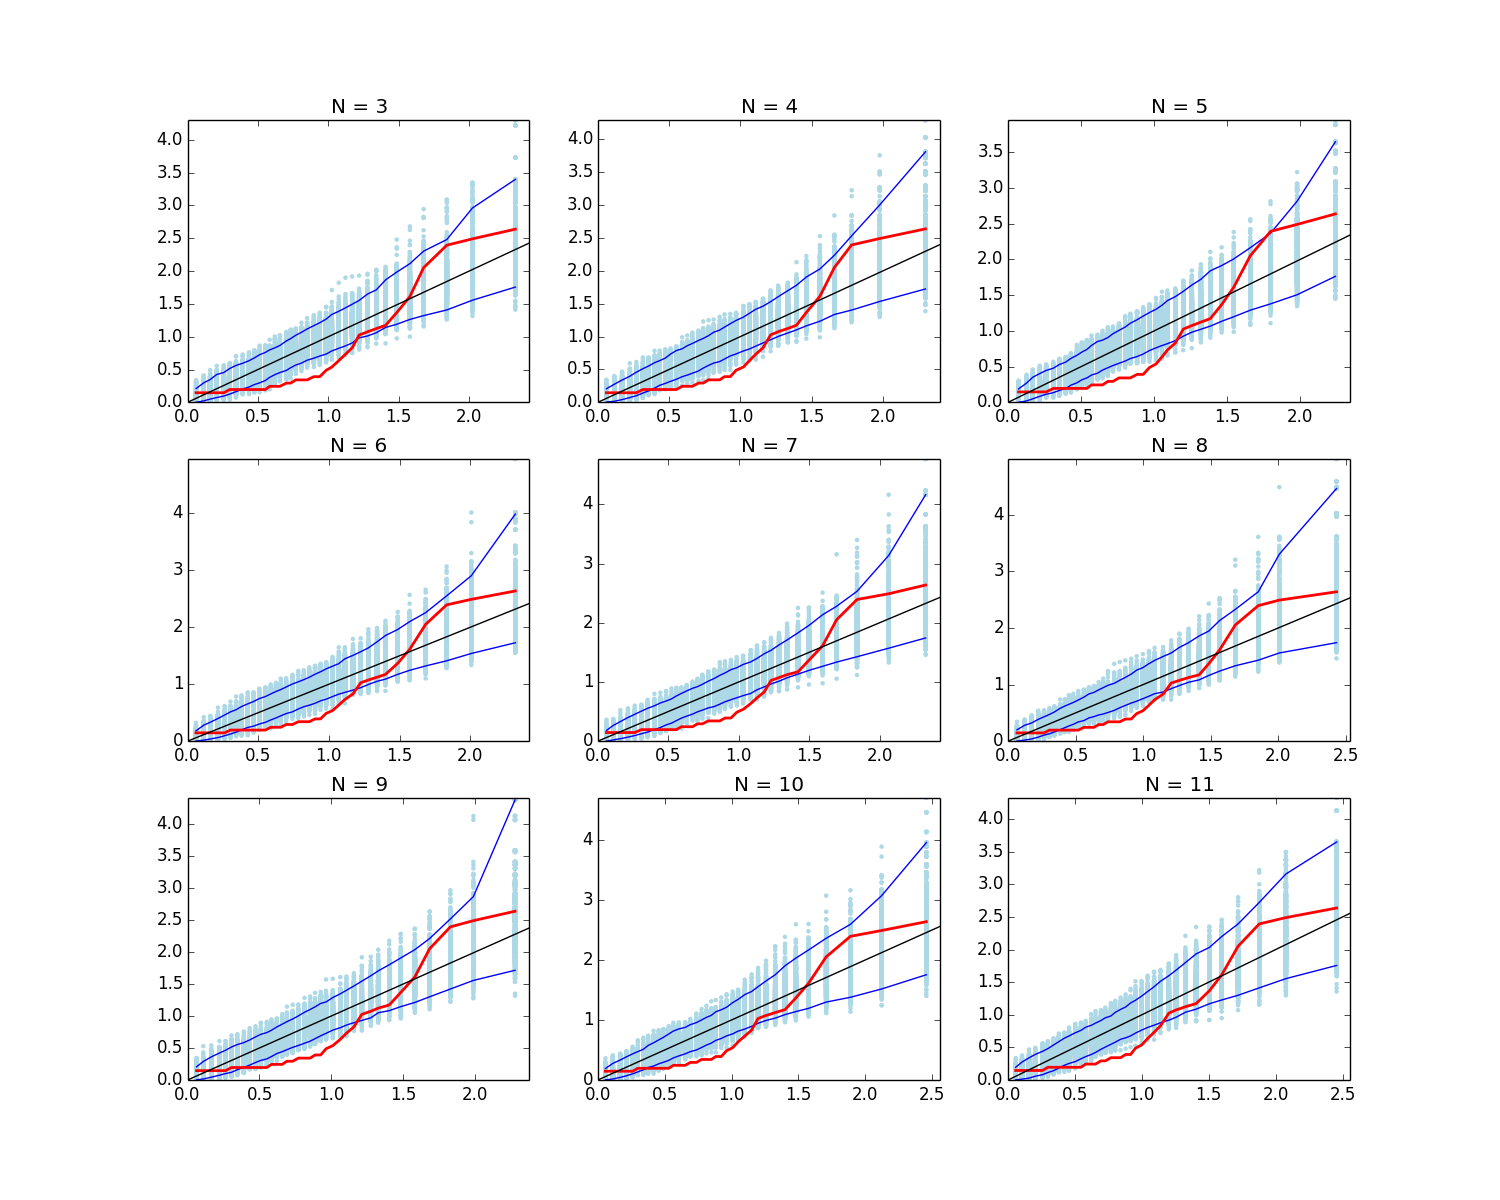
\includegraphics[width=0.5\textwidth]{17sept2015b-2-qq}}
  \caption{QQ plots for constant parameter model}
\end{figure}

In figure 2, we simulate the statistical model for 9 values of $N$, from 3 through 11, and display examples of a cell whose behavior is well-explained by this model and one whose behavior is not explained at all by this model, as indicated by the QQ plots. In fact, in 60 out of the 90 trials, the QQ plots indicated that the observed distribution remained within the 95\% confidence intervals at each quantile. However, we also note that in 19 out of the 90 trials, the tail of the distribution was above the identity line in the QQ plot. Thus, we have not yet completely explained the existence of high amplitudes with high probability yet.

% \begin{figure}
%   \caption{QQ plots of a good fit}
%   \centering
%   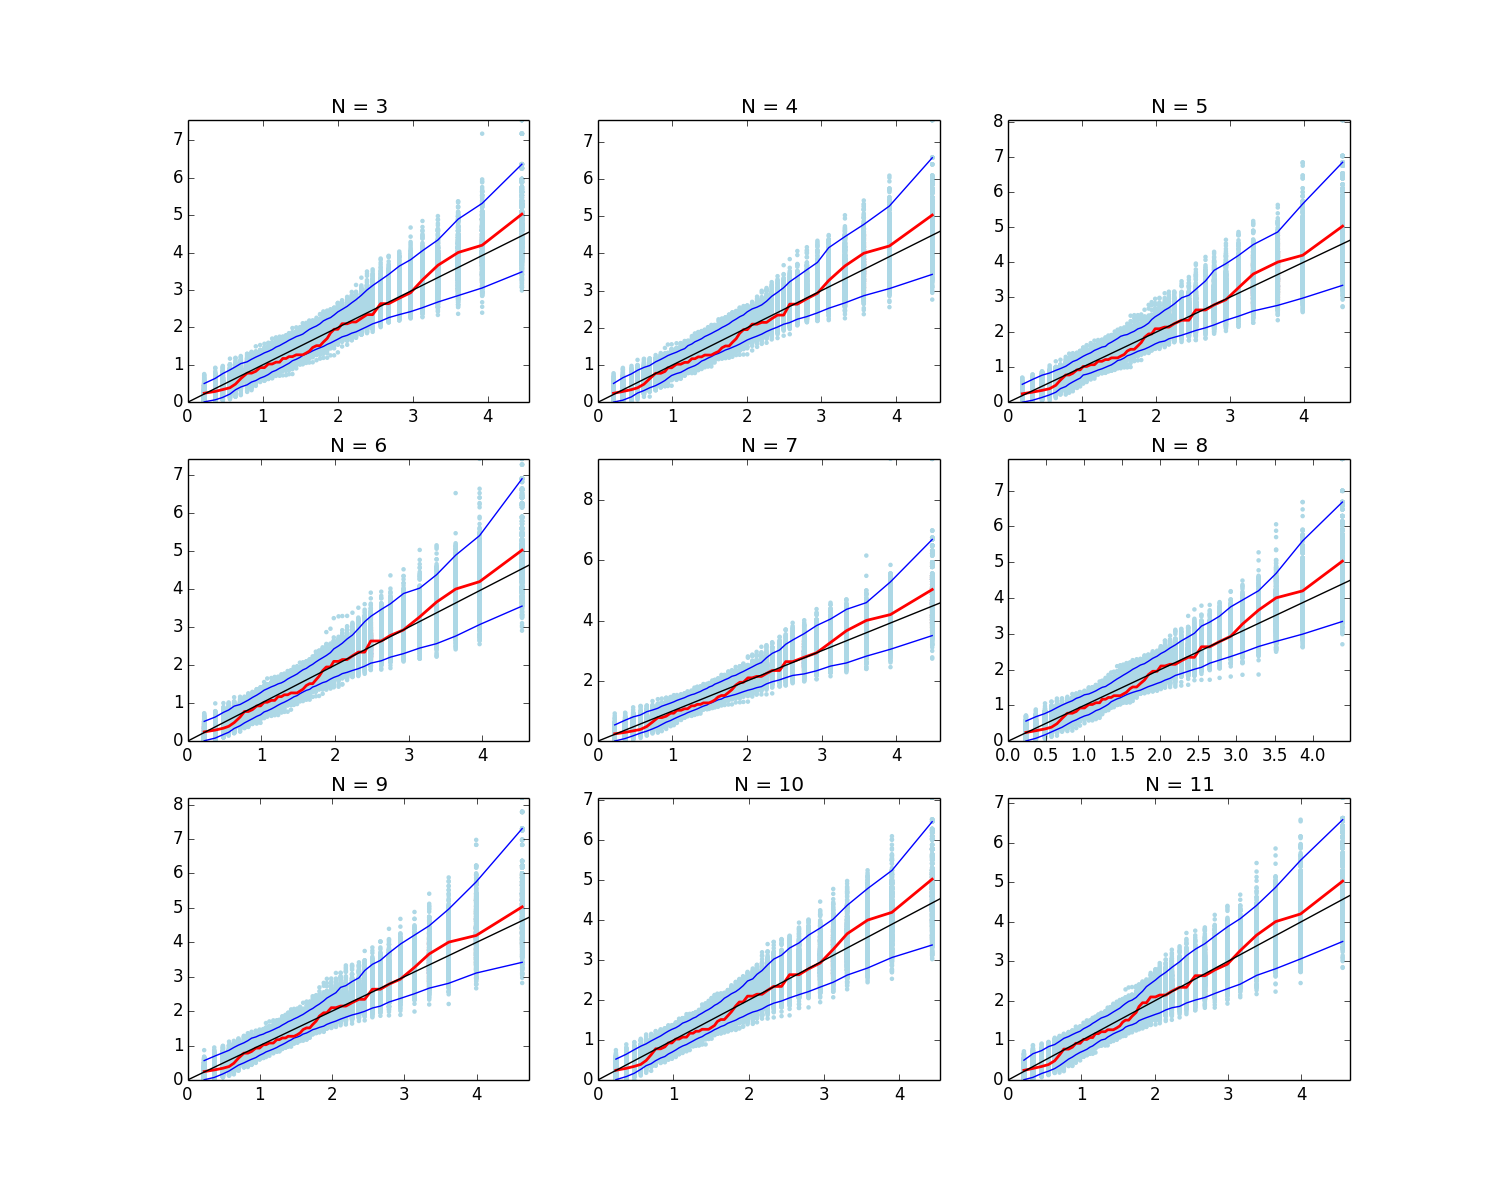
\includegraphics[width=0.8\textwidth]{11sept2015e-9-qq}
% \end{figure}
%
% \begin{figure}
%   \caption{QQ plots of a bad fit}
%   \centering
%   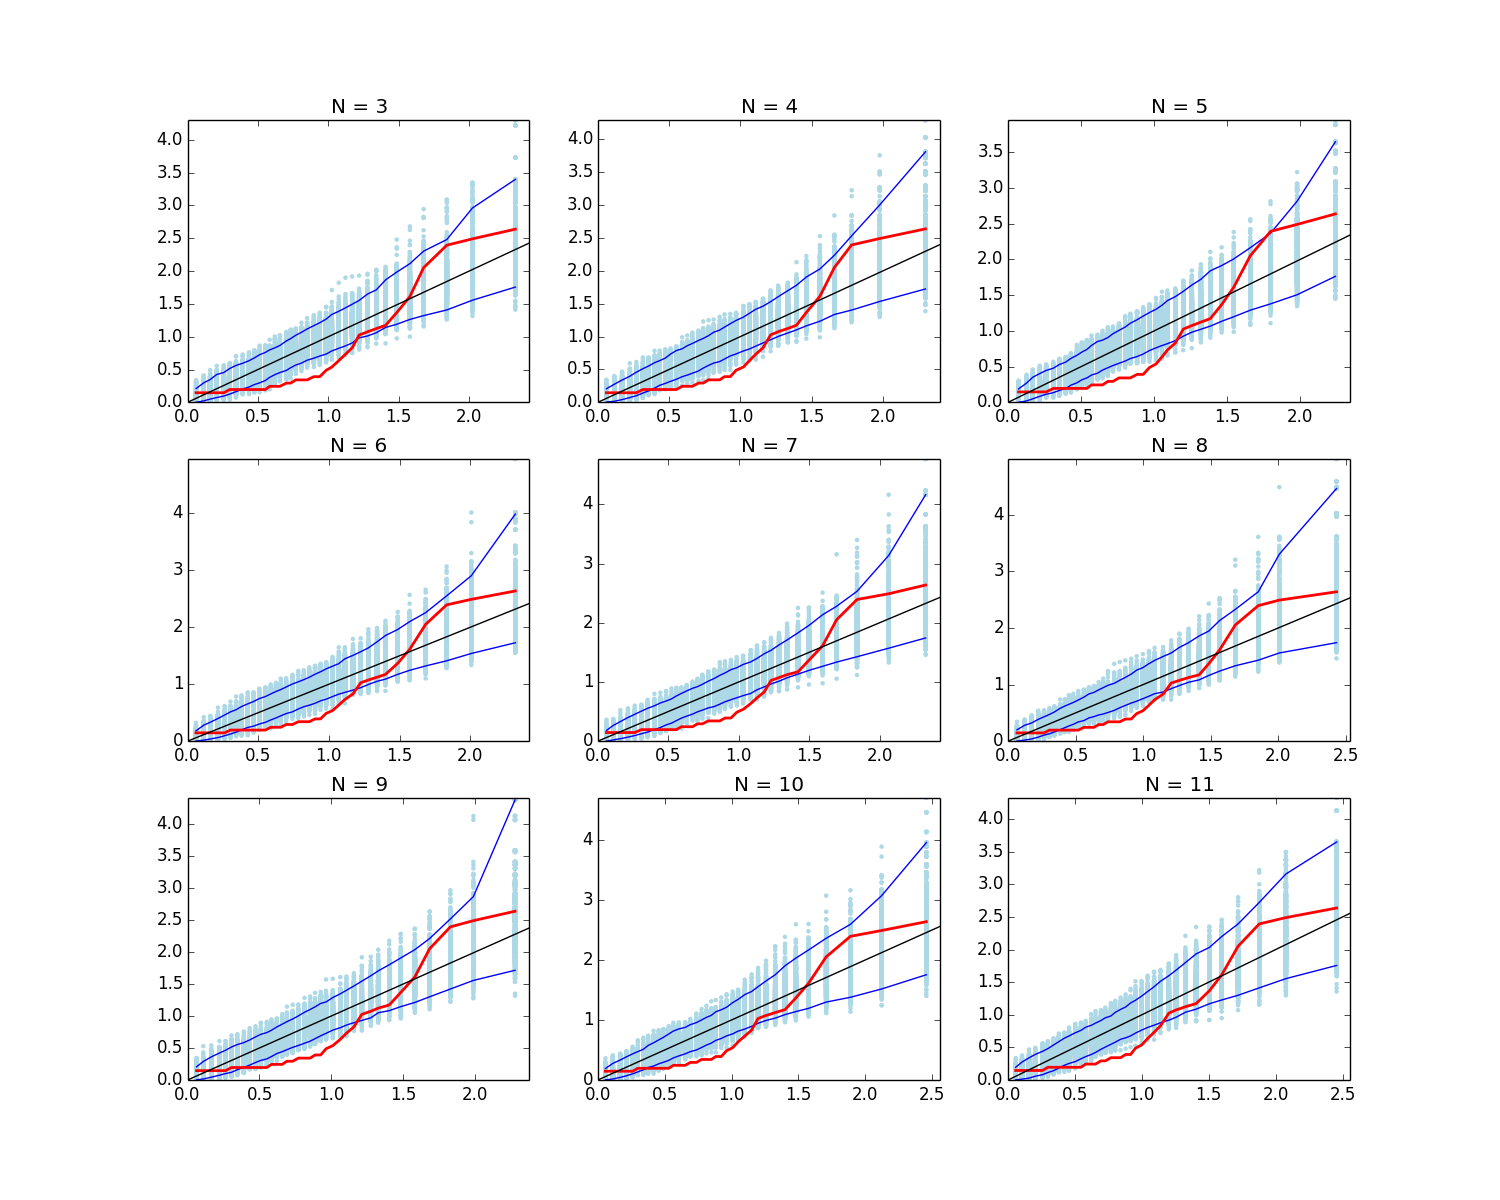
\includegraphics[width=0.8\textwidth]{17sept2015b-2-qq}
% \end{figure}

\subsection{Analysis of distributions on response amplitudes}
Equipped with a statistical model with parameters to explore, we attempt to explain the observed data by changing our assumptions on the parameters. We keep the mathematically convenient assumption of constant $p$ and $\sigma$ and assume distributions other than the point mass distribution on $q$. We begin with two distributions whose distribution is defined by its width and perturb its width to see the effect on the QQ plots.

\subsubsection{Uniform distribution}
In order to ensure that our statistical model has the same mean value, we take our uniform distribution with width $w$ to have the pdf
\[
  f_q(x) = 1_{\left[\frac{\overline{\mu}}{Np}-\frac12 w,\frac{\overline{\mu}}{Np}+\frac12 w\right]} \frac1{w}
\]
where $1_S$ is the indicator function for the set $S$. Since we restrict our response amplitudes to be positive, we simulate our distribution for a range of values of $w$ from the interval $\left[0,2\frac{\overline{\mu}}{Np}\right)$.

However, even at the widest possible interval for the uniform distribution, significant imporvements in the QQ plot were not observed.

\subsubsection{Arcsine distribution}
We similarly attempted an arcsine distribution, which specifies more weight on the highest and lowest amplitudes in the given width. Similarly, we did not observe significants improvements, though better than the uniform distribution.

\subsection{Curve fitting of the cdf}
We first show that we can express the cdf of $\rv{A}$ as a sum of Gaussians cdfs as follows. We observe an amplitude of $\sum_{j\in S} N(q_j,\sigma^2) = N\left(\sum_{j\in S} q_j, \vert S\vert\sigma^2\right)$ with probability $\prod_{j\in S} p = p^{\vert S\vert}$, where $S\subseteq [N]$ is a set of indices of synaptic contacts and $[N]$ denotes the set $\{1,2,\dots, N\}$. Thus, the pdf of the overall distribution is
\[
  f_{\rv{A}}(x) = \sum_{S\in \mathcal{P}([N])} p^{\vert S\vert} \varphi_{\sum_{j\in S} q_j, \vert S\vert\sigma^2}(x).
\]
where $\mathcal{P}([N])$ denotes the power set of $[N]$ and $\varphi_{\mu,\sigma^2}(x)$ denotes the pdf of the Gaussian variable with mean $\mu$ and variance $\sigma^2$. Then, we have the cdf by integrating:
\[
  F_{\rv{A}}(x) = \int_0^x f_{\rv{A}}(t)\, dt = \int_0^x \sum_{S\in \mathcal{P}([N])} p^{\vert S\vert} \varphi_{\sum_{j\in S} q_j, \vert S\vert\sigma^2}(t)\, dt = \sum_{S\in \mathcal{P}([N])} p^{\vert S\vert} \left(\Phi_{\sum_{j\in S} q_j, \vert S\vert\sigma^2}(x) - \Phi_{\sum_{j\in S} q_j, \vert S\vert\sigma^2}(0)\right)
\]
where $\Phi_{\mu,\sigma^2}$ denotes the cdf of the Gaussian variable with mean $\mu$ and variance $\sigma^2$.

Now note that we have estimates of points $(x,F_{\rv{A}}(x))$ that the cdf satisfies, since we have observed amplitudes $x_i$ and an estimate of $F_{\rv{A}}(x_i)$ by sorting the observed amplitudes and taking the $i$th amplitude $x_i$ in the sorted data to have $F_{\rv{A}}(x_i) = \frac1{i+1}$. In fact, this is equivalent to fitting the quantiles of $F_{\rv{A}}(x)$ to match the data as in the QQ plot analysis.

\section{Methods/Technical Appendix}
\subsection{Estimation of pararmeters for constant parameter model}
\subsubsection{Release probability}
Under any assumption of the parameters, we have that the postsynaptic amplitude is 0 if and only if all $N$ contacts are 0. Then, if we assume that all the $p_j$ are equal, then we can express the probability that the postsynaptic amplitude is 0 as
\[
  \Pr[\rv{A} = 0] = (1-p)^N.
\]
We have an empirical estimate for $\Pr[\rv{A} = 0]$, the failure rate, which we write as $p_f$. Then, we can estimate $p$ as
\[
  p_f = (1-p)^N \iff p = 1 - \sqrt[N]{p}.
\]

\subsubsection{Response amplitude}
Suppose that $p$ and $q$ are constant across all contacts. Then, by linearity of expectation, we have that
\begin{align*}
  \E[\rv{A}] &= \sum_{j=1}^N \E[\rv{A}_j] \\
  &= \sum_{j=1}^N \E[\rv{A}_j\mid \rv{S}_j = 1]\Pr[\rv{S}_j = 1] + \E[\rv{A}_j\mid \rv{S}_j = 0]\Pr[\rv{S}_j = 0] \\
  &= \sum_{j=1}^N \E[N(q,\sigma^2)]p + 0 = \sum_{j=1}^N qp = Nqp.
\end{align*}
Then, since we already have an estimate for $p$ and we can find an estimate for $\E[\rv{A}]$ by taking the average value $\overline{\mu}$ of all our observations, we have that
\[
  \overline{\mu} = Nqp \iff q = \frac{\overline{\mu}}{Np}.
\]

\subsubsection{Variance}
Since we assumed that the $\rv{A}_j$ are independent, we have, by the linearity of variance for independent random variables, that
\begin{align*}
  \Var[\rv{A}] &= \sum_{j=1}^N \Var[\rv{A}_j] \\
  &= \sum_{j=1}^N \E[\rv{A}_j^2] - \E[\rv{A}_j]^2 \\
  &= \sum_{j=1}^N \E[\rv{A}_j^2\mid \rv{S}_j = 1]\Pr[\rv{S}_j = 1] + \E[\rv{A}_j^2\mid \rv{S}_j = 0]\Pr[\rv{S}_j = 0] - \E[\rv{A}_j]^2 \\
  &= \sum_{j=1}^N (\sigma^2 + q^2)p + 0 - q^2p^2 \\
  &= N(\sigma^2p + q^2p - q^2p^2).
\end{align*}
Again, we have an empirical estimate of $\Var[\rv{A}]$, the sample variance $s^2$, so we can estimate $\sigma^2$ as
\[
  s^2 = N(\sigma^2p + q^2p - q^2p^2) \iff \sigma^2 = \frac{s^2}{Np} - q^2 + q^2p.
\]

\subsection{Estimation of parameters for distributed response model}
Under this model, the release probabilities are still taken to be constant so we use the same estimation of release probability as the above.

\subsubsection{Response amplitude}
In order to make a suitable choice of the $q_j$, we simply require that the mean of the model matches the mean of the observed data. Note that we can enforce this by restricting the average value of the $q_j$, since
\[
  \overline{\mu} = \sum_{j=1}^N p_jq_j = p\sum_{j=1}^N q_j \iff \frac1{N} \sum_{j=1}^N q_j = \frac{\overline{\mu}}{Np}.
\]

For both the uniform and arcsine distributions, the mean of the distribution is given by $\frac12 (a+b)$ where the support of the distribution is $[a,b]$. Furthermore, the distribution is completely determined by the support of the distribution for both the uniform and arcsine distributions. Thus, we determine $a$ and $b$ given this requirement in addition to the assumed value of the width $w$ of the distribution, which is simply $w = b - a$:
\[
  \begin{pmatrix}\frac12&\frac12\\-1&1\end{pmatrix} \begin{pmatrix}a\\b\end{pmatrix} = \begin{pmatrix}\frac{\overline{\mu}}{Np}\\w\end{pmatrix} \iff \begin{pmatrix}a\\b\end{pmatrix} = \begin{pmatrix}1&-\frac12\\1&\frac12\end{pmatrix} \begin{pmatrix}\frac{\overline{\mu}}{Np}\\w\end{pmatrix} = \begin{pmatrix}\frac{\overline{\mu}}{Np}-\frac12 w\\ \frac{\overline{\mu}}{Np}+\frac12 w\end{pmatrix}.
\]
Thus, we derive the uniform distribution pdf
\[
  f_q(x) = 1_{S} \frac1{w}
\]
and the arcsine distribution pdf
\[
  f_q(x) = 1_{S} \frac1{\pi\sqrt{(x-(\frac{\overline{\mu}}{Np}-\frac12 w))((\frac{\overline{\mu}}{Np}+\frac12 w)-x)}}
\]
where $1_S$ is the indicator function for $\left[\frac{\overline{\mu}}{Np}-\frac12 w,\frac{\overline{\mu}}{Np}+\frac12 w\right]$.

\subsubsection{Variance}
When we do not assume constant $q$, we modify the previous argument slighty.
\begin{align*}
  \Var[\rv{A}] &= \sum_{j=1}^N \E[\rv{A}_j^2\mid \rv{S}_j = 1]\Pr[\rv{S}_j = 1] + \E[\rv{A}_j^2\mid \rv{S}_j = 0]\Pr[\rv{S}_j = 0] - \E[\rv{A}_j]^2 \\
  &= \sum_{j=1}^N (\sigma^2 + q_j^2)p + 0 - q_j^2p^2 \\
  &= N\sigma^2p + \sum_{j=1}^N q_j^2(p - p^2).
\end{align*}
As before, we use the sample variance $s^2$, to estimate $\sigma^2$ as
\[
  s^2 = N\sigma^2p + \sum_{j=1}^N q_j^2(p - p^2) \iff \sigma^2 = \frac{s^2}{Np} - \frac{1-p}{N}\sum_{j=1}^N q_j^2.
\]

\end{document}
